\documentclass[12pt, titlepage]{article}

\usepackage{fullpage}
\usepackage[round]{natbib}
\usepackage{multirow}
\usepackage{booktabs}
\usepackage{tabularx}
\usepackage{float}
\usepackage{amsfonts}
\usepackage{graphicx}
\usepackage{float}
\usepackage{hyperref}
\hypersetup{
    colorlinks,
    citecolor=black,
    filecolor=black,
    linkcolor=red,
    urlcolor=blue
}
\usepackage[round]{natbib}

\newcounter{acnum}
\newcommand{\actheacnum}{AC\theacnum}
\newcommand{\acref}[1]{AC\ref{#1}}

\newcounter{ucnum}
\newcommand{\uctheucnum}{UC\theucnum}
\newcommand{\uref}[1]{UC\ref{#1}}

\newcounter{mnum}
\newcommand{\mthemnum}{M\themnum}
\newcommand{\mref}[1]{M\ref{#1}}

\title{SE 3XA3: Software Requirements Specification\\Poker Project}

\author{Team 12
        \\ Safwan Hossain and hossam18
        \\ Eamon Earl and earle2
        \\ Tyler Magarelli and magarelt
}

\date{March 18, 2022}

% \input{../../Comments}

\begin{document}

\maketitle

\pagenumbering{roman}
\tableofcontents
\listoftables
\listoffigures

\begin{table}[bp]
\caption{\bf Revision History}
\begin{tabularx}{\textwidth}{p{3cm}p{2cm}X}
\toprule {\bf Date} & {\bf Version} & {\bf Notes}\\
\midrule
March 16, 2022 & 1.0 & Initial Draft\\
March 18, 2022 & 1.1 & Revised Draft\\
\bottomrule
\end{tabularx}
\end{table}

\newpage

\pagenumbering{arabic}

\section{Introduction}

\subsection{Summary of Project}

Our Poker Project is aptly named; we aim to build upon a relatively primitive base code for evaluating poker hand states and create a fully playable online poker experience. Our main motivation behind developing this software is to remove the barriers that other similar products have neglected to in the past, namely the requirement of financial commitment from the user. We firmly believe in the educational and developmental value of a strategic, high-stakes main.model.game like poker, but we also believe that losing money and promoting detrimental habits and addiction are not inherent to that high-stakes feeling. Our project will make this main.model.game accessible to students and other young people who are not in the financial situation to regularly go to a casino or use a monetary gambling app, and will give them the opportunity to develop valuable risk analysis skills and have fun with their friends, without the chance of harming their future.

\subsection{Context of Module Guide}

This document underlines the distinctions made using the information gathered from the requirements document, and how they will go on to partition the elements of the software into distinct modules, which are described in detail in the MIS below (Section 8). We have also developed traceability matrices to ensure that we have both encapsulated all of our required behaviour somewhere within the specification of the current architecture, and that our anticipated changes will have a "future home" as well. This document will provide various views on where we are currently at in the development process, where we were and where we intend on going, such that it will have some inherent value to each stakeholder involved. These include:

\begin{itemize}
    \item Designers: This document will act as an oracle for the design and dependencies of the programs to be written by the development team, showing both what is expected and likely areas of faults or stress, so that the designers can reinforce the importance of those areas and ensure that the developers are implementing them correctly. It also acts as information hiding, so when verifying the final product the design team can simply refer to the overarching hierarchy and behaviour described by the MIS, as opposed to reading through the code or its associated documentation. Additionally, as designing for generality is a specific property that we have prioritized given the possible application of the software to additional card main.model.game simulations, and we have already begun the process of considering anticipated changes, it allows the designers to freely consider what areas of the program may have the flexibility to accommodate for these heuristics.
    \item Developers: The viewpoint of this document that is most applicable to the developers is that of the MIS; the technical specification of what each module and their encapsulated routines must achieve. If the designers are vigilant and the requirements are fully and unambiguously specified, the developer should not have to consider anything else. Regardless, the abstraction of the architecture is there for their consideration, and interfacing directly with the source code may also give them unique insight into areas for achieving the previously discussed heuristics of generality and modifiability.
    \item Clients: The clients can use this document as a metric of the degree to which their business requirements are being met, specifically with Sections 4 and 6. They can also validate whether or not any anticipated changes conflict with any of their prior expectations, or if any unlikely changes highlight new behaviour that they may want to reconsider. However, it must be acknowledged that prioritizing a change after it has already been deemed unlikely may inherently cause some code overhaul and some setback in the lifetime of the development.  
\end{itemize}

\subsection{Design Principles}

As previously discussed, the main principles we are hoping to achieve with our design are generality and modifiability / designing for change. This is based off of the principle that the lifespan of our project is relatively small and consequently so is the scope, and as such there is very likely to be further development on this code in the future with the addition of further features and main.model.game modes, just as this project was based and developed on top of some previous source code; such is the nature and the beauty of open source projects. These principles encapsulate other ones, however, which can be seen throughout our design. Modularity is a principle that boils down parts of the functional source code into the smallest, distinct sections, which we have designed to have high internal coupling and low cohesion with other such modules. This allows for a module to be swapped out with another in the future, with minimal effects on the rest of the program. We also designed our program following the MVC (Model-main.view.View-Controller) architecture, which inherently partitions the program into three main sections, such that concerns can be separated when working in each distinct region. It also distinguishes areas of the code that are most important to different stakeholders and for different purposes. The data main.model will be used as a base for the current main.model.game mode and all future main.model.game modes, while the main.view is the most important section when considering the user. The controllers act as individual scripts for each main.model.game mode, and the main.server.Server works to trigger the controllers and link communication between multiple clients. All of these abstracted sections connect with the rest of the system minimally, ensuring that changes to the system can be made easily.

\subsection{Outline}

The rest of the document is organized as follows. Section
\ref{SecChange} lists the anticipated and unlikely changes of the software
requirements. Section \ref{SecMH} summarizes the module decomposition that
was constructed according to the likely changes. Section \ref{SecConnection}
specifies the connections between the software requirements and the
modules. Section \ref{SecMD} gives a detailed description of the
modules. Section \ref{SecTM} includes two traceability matrices. One checks
the completeness of the design against the requirements provided in the SRS. The
other shows the relation between anticipated changes and the modules. Section
\ref{SecUse} describes the use relation between modules.

\section{Anticipated and Unlikely Changes} \label{SecChange}

This section lists possible changes to the system. According to the likeliness
of the change, the possible changes are classified into two
categories. Anticipated changes are listed in Section \ref{SecAchange}, and
unlikely changes are listed in Section \ref{SecUchange}.

\subsection{Anticipated Changes} \label{SecAchange}

Anticipated changes are the source of the information that is to be hidden
inside the modules. Ideally, changing one of the anticipated changes will only
require changing the one module that hides the associated decision. The approach
adapted here is called design for
change.

\begin{description}
\item[\refstepcounter{acnum} \actheacnum \label{acHardware}:] Using a higher fidelity main.server.
\item[\refstepcounter{acnum} \actheacnum \label{acInput}:] Implementing the chip betting system with preset chip values (5, 10, 20, 100, etc.)
\item[\refstepcounter{acnum} \actheacnum \label{acData}:] The format of the data that is exchanged between the clients and the main.server.
\item[\refstepcounter{acnum} \actheacnum \label{acSync}:] The method of how all clients synchronize gameplay.
\item[\refstepcounter{acnum} \actheacnum \label{acSync}:] The addition of a main.controller template, that all main.controller classes will implement, to make running various main.model.game modes from the same starting menu easier.
\item[\refstepcounter{acnum} \actheacnum \label{acSync}:] main.view.GameView will be developed to have more useful display functionality, to relieve some complication of scripting gameplay in the main.controller, improving readability and fixing some cohesion issues.
\end{description}

\subsection{Unlikely Changes} \label{SecUchange}

%DELETE
The module design should be as general as possible. However, a general system is
more complex. Sometimes this complexity is not necessary. Fixing some design
decisions at the system architecture stage can simplify the software design. If
these decision should later need to be changed, then many parts of the design
will potentially need to be modified. Hence, it is not intended that these
decisions will be changed.

\begin{description}
\item[\refstepcounter{ucnum} \uctheucnum \label{ucIO}:] Input/Output devices (Input: File and/or Keyboard, Output: File, Memory, and/or Screen).
\item[\refstepcounter{ucnum} \uctheucnum \label{ucInput}:] There will always be a source of input data external to the software.
\item[\refstepcounter{ucnum} \uctheucnum:] A main.server will always be used for every main.model.game.
\item[\refstepcounter{ucnum} \uctheucnum:] The main.model for the deck will not change.
\end{description}

\section{Module Hierarchy} \label{SecMH}

This section provides an overview of the module design. Modules are summarized
in a hierarchy decomposed by secrets in Table \ref{TblMH}. The modules listed
below, which are leaves in the hierarchy tree, are the modules that will
actually be implemented.

\begin{description}
\item [\refstepcounter{mnum} \mthemnum \label{mHH}:] Hardware-Hiding Module
\item [\refstepcounter{mnum} \mthemnum \label{mModel}:] Model Module
\item [\refstepcounter{mnum} \mthemnum \label{mView}:] main.view.View Module
\item [\refstepcounter{mnum} \mthemnum \label{mController}:] Controller Module
\end{description}


\begin{table}[H]
\centering
\begin{tabular}{p{0.3\textwidth} p{0.6\textwidth} }
\toprule
\textbf{Level 1} & \textbf{Level 2}\\
\midrule

{Hardware-Hiding Module} & ~ \\
\midrule

\multirow{12}{0.3\textwidth}{Model Module} 
& main.model.client.Client\\
& main.model.update.GameInfo\\
& main.server.Server\\
& main.model.game.Game\\
& main.model.player.Card\\
& main.model.player.Player\\
& main.util.HandEvaluator\\
& main.model.player.Deck\\
& main.enumeration.main.model.game.PlayerAction\\
\midrule

\multirow{2}{0.3\textwidth}{main.view.View Module}
& main.view.MainMenuView\\
& main.view.GameView\\
\midrule 

\multirow{3}{0.3\textwidth}{Controller Module} 
& main.controller.MainController\\
& main.controller.ClientControllerOld\\
& main.server.ClientHandler\\
\bottomrule

\end{tabular}
\caption{Module Hierarchy}
\label{TblMH}
\end{table}

\section{Connection Between Requirements and Design} \label{SecConnection}


The design for this system is intended to meet all the requirements established in the first SRS document. The system is broken down into modules that will have their own requirements and when the modules are put together, the system will satisfy all of the requirements. Table 1 shows the relationship between needs and modules. \ref{TblRT}.

\section{Module Decomposition} \label{SecMD}

Modules are decomposed according to the principle of ``information hiding''
proposed by \citet{ParnasEtAl1984}. The \emph{Secrets} field in a module
decomposition is a brief statement of the design decision hidden by the
module. The \emph{main.util.Services} field specifies \emph{what} the module will do
without documenting \emph{how} to do it. For each module, a suggestion for the
implementing software is given under the \emph{Implemented By} title. If the
entry is \emph{OS}, this means that the module is provided by the operating
system or by standard programming language libraries.  Also indicate if the
module will be implemented specifically for the software.

Only the leaf modules in the
hierarchy have to be implemented. If a dash (\emph{--}) is shown, this means
that the module is not a leaf and will not have to be implemented. Whether or
not this module is implemented depends on the programming language
selected.

% ========== HARDWARE ========== %
\subsection{Hardware Hiding Modules (\mref{mHH})}

\begin{description}
\item[Secrets:]The data structure and algorithm used to implement the virtual
  hardware.
\item[main.util.Services:]Serves as a virtual hardware used by the rest of the
  system. This module provides the interface between the hardware and the
  software. So, the system can use it to display outputs or to accept inputs.
\item[Implemented By:] OS
\end{description}

% ========== MODEL ========== %

\subsection{Model Module}
    \begin{description}
    \item[Secrets:] Decides how elements of main.model.game data will stored and updated.
    \item[main.util.Services:] This module will determine the structure of majority of the system. It will consist of all the data elements that will need to be stored in order to run the program and modules that will implement functions that determine how the data can be updated.
    \item[Implemented By:] --
    \end{description}

\subsubsection{ main.model.client.Client Module (\mref{mModel})}
    \begin{description}
    \item[Secrets:] The information and components for a user to interact with the main.server.
    \item[main.util.Services:] Stores information about the user that is needed by the main.server to identify and manipulate each unique client.
    \item[Implemented By:] main.controller.ClientControllerOld
    \end{description}

\subsubsection{ main.model.update.GameInfo Module (\mref{mModel})}
    \begin{description}
    \item[Secrets:] Decides how to store main.model.game data.
    \item[main.util.Services:] Stores important main.model.game data that will be communicated between a main.server and client.
    \item[Implemented By:] main.model.client.Client, main.controller.ClientControllerOld, main.server.ClientHandler
    \end{description}

\subsubsection{ main.server.Server Module (\mref{mModel})}
    \begin{description}
    \item[Secrets:] Decides how to store and manage client and main.server data.
    \item[main.util.Services:] Stores main.server and client data, allowing users to establish a connection to the main.server.
    \item[Implemented By:] main.controller.MainController
    \end{description}

\subsubsection{ main.model.game.Game Module (\mref{mModel})}
    \begin{description}
    \item[Secrets:] Decides to store important elements of the main.model.game.
    \item[main.util.Services:] Provides a system to store and manage elements of the main.model.game that will keep track of the main.model.game's progress.
    \item[Implemented By:] main.controller.ClientControllerOld
    \end{description}

\subsubsection{ main.model.player.Card Module (\mref{mModel})}
    \begin{description}
    \item[Secrets:] Stores information about a card.
    \item[main.util.Services:] Provides a way to store a card suite and rank in a single data type.
    \item[Implemented By:] main.model.game.Game, main.model.player.Deck
    \end{description}

\subsubsection{ main.model.player.Player Module (\mref{mModel})}
    \begin{description}
    \item[Secrets:] Stores information about a player.
    \item[main.util.Services:] Provides a way to store and represent each player of the main.model.game.
    \item[Implemented By:] main.model.game.Game
    \end{description}

\subsubsection{ main.util.HandEvaluator Module (\mref{mModel})}
    \begin{description}
    \item[Secrets:] Decides the card rankings of each player's hand.
    \item[main.util.Services:] Provides a way to assign each player a hand ranking for comparison.
    \item[Implemented By:] main.model.game.Game
    \end{description}

\subsubsection{ main.model.player.Deck Module (\mref{mModel})}
    \begin{description}
    \item[Secrets:] Stores information about a deck of cards
    \item[main.util.Services:] Provides functions and storage for a collection of cards.
    \item[Implemented By:] main.model.game.Game
    \end{description}
    
\subsubsection{ main.enumeration.main.model.game.PlayerAction Module (\mref{mModel})}
    \begin{description}
    \item[Secrets:] Stores information about valid main.model.game moves.
    \item[main.util.Services:] Provides a way to validate user inputs by confirming if their input is a valid main.model.game move.
    \item[Implemented By:] main.model.game.Game, main.model.update.GameInfo, main.server.ClientHandler, main.model.client.Client
    \end{description}
% ========== VIEW ========== %

\subsection{main.view.View Module}
    \begin{description}
    \item[Secrets:] Decides how elements of main.model.game data will be displayed to the user.
    \item[main.util.Services:] This module will provide the visual aspect of the program, providing modules that will allow the data in the program to be displayed to the user in a meaningful way. Almost all elements of the main.view module will be easily modifiable with minimal collateral to other code.
    \item[Implemented By:] --
    \end{description}

\subsubsection{ main.view.MainMenuView Module (\mref{mView})}
    \begin{description}
    \item[Secrets:] Decides how the main menu of the program will be displayed.
    \item[main.util.Services:] Provides a way to display and navigate the main menu. Also contains error and success messages.
    \item[Implemented By:] main.controller.MainController
    \end{description}
    
\subsubsection{ main.view.GameView Module (\mref{mView})}
    \begin{description}
    \item[Secrets:] Decides how the main.model.game will be visually represented to the user.
    \item[main.util.Services:] Provides a way to display all the elements of the main.model.game to the user in a meaningful way. Also contains error and success messages.
    \item[Implemented By:] main.controller.ClientControllerOld
    \end{description}

% ========== CONTROLLER ========== %

\subsection{Controller Module}

\begin{description}
\item[Secrets:] Decides and handles the software decision making process. When and what data will be manipulated by user input.
\item[main.util.Services:] This module will act as a mediator between the main.view, main.model and the user. It will utilize the main.view and the main.model to display data to the user and take in user input and decide how the user input will manipulate the data.
\item[Implemented By:] --
\end{description}

\subsubsection{ main.controller.MainController Module (\mref{mController})}
    \begin{description}
    \item[Secrets:] Decides how to enter and setup the main.model.game.
    \item[main.util.Services:] Provides an interface to users on how to set up and join a main.model.game.
    \item[Implemented By:] Hardware-Hiding Module
    \end{description}

\subsubsection{ main.controller.ClientControllerOld Module (\mref{mController})}
    \begin{description}
    \item[Secrets:] Decides how the user can manipulate main.model.game data according to a central main.server consisting of multiple players.
    \item[main.util.Services:] Acts as the "brain" of the program by providing a synchronous way to play the main.model.game with other online players.
    \item[Implemented By:] Hardware-Hiding Module
    \end{description}

\subsubsection{ main.server.ClientHandler Module (\mref{mController})}
    \begin{description}
    \item[Secrets:] Decides how the main.server should respond to user input.
    \item[main.util.Services:] Provides a way for users to communicate with the main.server behind the scenes
    \item[Implemented By:] Hardware-Hiding Module
    \end{description}

% ======== PART 6 ======== %


\section{Traceability Matrix} \label{SecTM}

This section shows two traceability matrices: between the modules and the
requirements and between the modules and the anticipated changes.

% the table should use mref, the requirements should be named, use something
% like fref
\begin{table}[H]
\centering
\begin{tabular}{p{0.2\textwidth} p{0.6\textwidth}}
\toprule
\textbf{Func. Req.} & \textbf{Modules}\\
\midrule
FR1 & \mref{mModel}, \mref{mView}\\
FR2 & \mref{mModel}, \mref{mView}\\
FR3 & \mref{mModel}, \mref{mView}\\
FR4 & \mref{mModel}, \mref{mView}, \mref{mController}\\
FR5 & \mref{mModel}, \mref{mController}\\
FR6 & \mref{mModel}, \mref{mController}\\
FR7 & \mref{mModel}\\
FR8 & \mref{mModel}\\
FR9 & \mref{mModel}\\
FR10 & \mref{mModel}, \mref{mView}, \mref{mController}\\
FR11 & \mref{mModel}, \mref{mView}\\
FR12 & \mref{mModel}, \mref{mView}\\
FR13 &\mref{mModel}, \mref{mView}, \mref{mController}\\
FR14 & \mref{mModel}, \mref{mView}, \mref{mController}\\
FR15 & \mref{mModel}, \mref{mView}, \mref{mController}\\
FR16 & \mref{mModel}, \mref{mView}, \mref{mController}\\
FR17 & \mref{mModel}, \mref{mController}\\
FR18 & \mref{mModel}, \mref{mController}\\
FR19 & \mref{mController}\\
FR20 & \mref{mModel}, \mref{mView}, \mref{mController}\\
FR21 & \mref{mModel}, \mref{mView}, \mref{mController}\\
FR22 & \mref{mModel}, \mref{mView}, \mref{mController}\\
FR23 & \mref{mModel}, \mref{mView}\\
FR24 & \mref{mModel}, \mref{mView}\\
FR25 & \mref{mModel}, \mref{mView}, \mref{mController}\\
FR26 & \mref{mModel}, \mref{mView}, \mref{mController}\\
FR27 & \mref{mModel}, \mref{mView}, \mref{mController}\\
FR28 & \mref{mModel}, \mref{mController}\\
FR29 & \mref{mModel}, \mref{mController}\\
FR30 & \mref{mModel}, \mref{mController}\\
\bottomrule
\end{tabular}
\caption{Trace Between Functional Requirements and Modules}
\label{TblRT}
\end{table}

\begin{table}[H]
\centering
\begin{tabular}{p{0.2\textwidth} p{0.6\textwidth}}
\toprule
\textbf{Non-Func. Req.} & \textbf{Modules}\\
\midrule
NFR1 & \mref{mHH}, \mref{mView}\\
NFR2 & \mref{mHH}\\
NFR3 & \mref{mHH}\\
NFR4 & \mref{mHH}, \mref{mController}\\
NFR5 & \mref{mHH}\\
NFR6 & \mref{mModel}, \mref{mController}\\
NFR7 & \mref{mHH}\\
NFR8 & \mref{mHH}\\
NFR9 & \mref{mHH}\\
NFR10 & \mref{mHH}\\
NFR11 & \mref{mHH}\\
NFR12 & \mref{mHH}, \mref{mController}\\
NFR13 & \mref{mHH}, \mref{mController}\\
\bottomrule
\end{tabular}
\caption{Trace Between Non-Functional Requirements and Modules}
\label{TblRT}
\end{table}

\begin{table}[H]
\centering
\begin{tabular}{p{0.2\textwidth} p{0.6\textwidth}}
\toprule
\textbf{AC} & \textbf{Modules}\\
\midrule
AC1 & \mref{mHH}\\
AC2 & \mref{mModel}\\
AC3 & \mref{mHH}\\
AC4 & \mref{mHH}\\
AC5 & \mref{mController}\\
AC6 & \mref{mView}, \mref{mController}\\
\bottomrule
\end{tabular}
\caption{Trace Between Anticipated Changes and Modules}
\label{TblACT}
\end{table}

\section{Use Hierarchy Between Modules} \label{SecUse}

In this section, the uses hierarchy between modules is
provided. A uses relation between module A and module B is defined to be that module A is dependant of module B to function correctly. For example, if module A uses module B then the correct functioning of A depends upon the availability of a correct
implementation of B. Figure \ref{FigUH} illustrates the use relation between
the modules for this program. It can be seen that the graph is a directed acyclic graph. Each level of the hierarchy provides a testable and functional component of the system, and higher-level modules are effectively simpler since they rely on lower-level modules.

\begin{figure}[H]
\centering
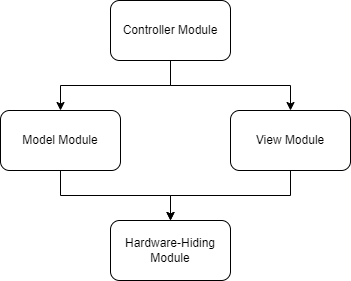
\includegraphics[width=0.7\textwidth]{Poker_UseDiagram.png}
\caption{Use hierarchy among modules}
\label{FigUH}
\end{figure}

\section{MIS}

\section* {main.model.player.Card (ADT)}

main.model.player.Card

\subsection* {Uses}

None

\subsection* {Syntax}

\subsubsection* {Imported Constants}

None

\subsubsection* {Imported Types}

None

\subsubsection* {Exported Access Programs}

\begin{tabular}{| l | l | l | p{5cm} |}
\hline
\textbf{Routine name} & \textbf{In} & \textbf{Out} & \textbf{Exceptions}\\
\hline
greater\verb|_|than & main.model.player.Card & $\mathbb{B}$ &\\
\hline
\end{tabular}

\subsection* {Semantics}

\subsubsection* {State Variables}

$\mathit{suit}: \text{I}$\\
$\mathit{rank}$: $\mathbb{I}$

\subsubsection* {State Invariant}

$1 <= \mathit{suit} <= 4$\\
$2 <= \mathit{rank} <= 14$

\subsubsection* {Assumptions}

None

\subsubsection* {Considerations}

None

\subsubsection* {Access Routine Semantics}

\noindent greater\verb|_|than(C):
\begin{itemize}
\item $rank >= C.rank \Longrightarrow true \phantom{a}|\phantom{a} false$ 

\end{itemize}

\section* {main.model.player.Player (ADT)}

main.model.player.Player

\subsection* {Uses}

main.model.player.Card

\subsection* {Syntax}

\subsubsection* {Imported Constants}

None

\subsubsection* {Imported Types}

main.model.player.Card

\subsubsection* {Exported Access Programs}

\begin{tabular}{| l | l | l | p{5cm} |}
\hline
\textbf{Routine name} & \textbf{In} & \textbf{Out} & \textbf{Exceptions}\\
\hline 
new main.model.player.Player & String, $\mathbb{I}$ & &\\
\hline
clear\verb|_|hand & & &\\
\hline
hasTurn & & $\mathbb{B}$ &\\
\hline 
giveTurn & & &\\
\hline 
takeTurn & & &\\
\hline 
set\verb|_|chips & $\mathbb{I}$ & &\\
\hline 
get\verb|_|chips & & $\mathbb{I}$ &\\
\hline 
take\verb|_|chips & $\mathbb{I}$ & & IllegalArgumentException\\
\hline 
insert & main.model.player.Card & &\\
\hline 
get\verb|_|hand & & main.model.player.Card [ ] &\\
\hline 
\end{tabular}

\subsection* {Semantics}

\subsubsection* {State Variables}

$\mathit{name}: String$\\
$\mathit{chips}: \mathbb{I}$ \\
$\mathit{hand} : \verb|main.model.player.Card [ ]|$\\
$has\verb|_|turn : \mathbb{B}$

\subsubsection* {State Invariant}

$0 <= \mathit{chips}$

\subsubsection* {Assumptions}

None

\subsubsection* {Considerations}

None

\subsubsection* {Access Routine Semantics}

\noindent new main.model.player.Player(s, c):
\begin{itemize}
\item transition : $hand, name, chips, has\verb|_|turn := \epsilon, s, c, False$ 
\end{itemize}

\noindent clear\verb|_|hand():
\begin{itemize}
\item transition : $hand := \epsilon$ 
\end{itemize}

\noindent hasTurn():
\begin{itemize}
\item return : $has\verb|_|turn$ 
\end{itemize}

\noindent giveTurn():
\begin{itemize}
\item transition : $has\verb|_|turn := True$ 
\end{itemize}

\noindent takeTurn():
\begin{itemize}
\item transition : $has\verb|_|turn := False$ 
\end{itemize}

\noindent set\verb|_|chips(c):
\begin{itemize}
\item transition : $chips := c$ 
\end{itemize}

\noindent get\verb|_|chips(c):
\begin{itemize}
\item return : $chips$ 
\end{itemize}

\noindent take\verb|_|chips(c):
\begin{itemize}
\item transition : $chips := chips - c$
\item error : $chips - c < 0 \Longrightarrow IllegalArgumentException$
\end{itemize}

\noindent insert(C):
\begin{itemize}
\item transition : $C \in hand$
\item post-condition: $\forall i \in [0..len(hand) - 2] : hand[i].rank <= hand[i+1].rank$ 
\item description : inserts the card C into hand such that the hand is ordered in ascending order by rank
\end{itemize}

\noindent get\verb|_|hand():
\begin{itemize}
\item return : $hand$ 
\end{itemize}

\section* {main.model.player.Deck (ADT)}

main.model.player.Deck

\subsection* {Uses}

main.model.player.Card
main.model.player.Player

\subsection* {Syntax}

\subsubsection* {Imported Constants}

None

\subsubsection* {Imported Types}

main.model.player.Card
main.model.player.Player

\subsubsection* {Exported Access Programs}

\begin{tabular}{| l | l | l | p{5cm} |}
\hline
\textbf{Routine name} & \textbf{In} & \textbf{Out} & \textbf{Exceptions}\\
\hline
fillDeck & & &\\
\hline
shuffle & & &\\
\hline 
reset & & &\\
\hline 
draw & $\mathbb{I}$& main.model.player.Card [ ] & StackOverflowException\\
\hline 
\end{tabular}

\subsection* {Semantics}

\subsubsection* {State Variables}

$\mathit{deck} : \verb|main.model.player.Card [52]|$\\
$\mathit{flop} : \verb|main.model.player.Card [ ]|$\\
$stack\verb|_|p : \mathbb{I}$

\subsubsection* {State Invariant}

$0 <= stack\verb|_|p <= 51$\\

\subsubsection* {Assumptions}

None

\subsubsection* {Considerations}

main.model.player.Deck is suggested to be implemented as a stack, but the choice is ultimately up to the development team. If it is not implemented as such, the stack\verb|_|p state variable will not be needed and its associated invariant can be disregarded.

\subsubsection* {Access Routine Semantics}

\noindent fill\verb|_|deck():
\begin{itemize}
\item transition : fills the deck stack with all 52 unique playing cards (of type main.model.player.Card)
\end{itemize}

\noindent shuffle():
\begin{itemize}
\item transition : randomly shuffles the current cards in the deck to a degree wherein the sequence can be expected to be drastically different from the precondition of the deck stack 
\end{itemize}

\noindent reset():
\begin{itemize}
\item transition : returns all 52 unique cards to the deck stack and shuffles the deck, s:= 0
\end{itemize}

\noindent draw(n):
\begin{itemize}
\item transition: removes the top n cards from the deck, and places them into a list 
\item exception: $n >$ remaining cards in the deck $\Longrightarrow StackOverflowException$
\item returns: main.model.player.Card [n]
\end{itemize}

\section*{main.model.game.Game}

main.model.game.Game

\subsection* {Uses}

main.model.player.Card
main.model.player.Player
main.model.player.Deck

\subsection* {Syntax}

\subsubsection* {Imported Constants}

None

\subsubsection* {Imported Types}

main.model.player.Card
main.model.player.Player
main.model.player.Deck

\subsubsection* {Exported Access Programs}

\begin{tabular}{| l | l | l | p{5cm} |}
\hline
\textbf{Routine name} & \textbf{In} & \textbf{Out} & \textbf{Exceptions}\\
\hline
new main.model.game.Game & main.model.player.Player [ ], $\mathbb{I}$ & &\\
\hline
startGame & $\mathbb{I}$ & &\\
\hline 
removePlayer & main.model.player.Player & &\\
\hline 
foldPlayer & main.model.player.Player & &\\
\hline 
is\verb|_|round\verb|_|over & & $\mathbb{B}$ &\\
\hline 
dealCards & $\mathbb{I}$ & &\\
\hline
getNextPlayer & & main.model.player.Player & RuntimeException\\
\hline 
getCurrentPlayer & & main.model.player.Player & RuntimeException\\
\hline 
giveNextTurn & & &\\
\hline
\end{tabular}

\subsection* {Semantics}

\subsubsection* {State Variables}

\begin{itemize}
    \item deck : main.model.player.Deck
    \item players: main.model.player.Player [ ]
    \item unfoldedPlayers: main.model.player.Player [ ]
    \item currentPlayerIndex: $\mathbb{I}$
    \item nextPlayerIndex: $\mathbb{I}$
    \item minimumCallAmount: $\mathbb{I}$
    \item round\verb|_|over: $\mathbb{B}$
\end{itemize}

\subsubsection* {State Invariant}

\begin{itemize}
    \item there must always be a number of unfolded players less than or equal to the number of players
    \item currentPlayerIndex must always be greater than or equal to 0 and less than the length of unfoldedPlayers
    \item same as above, but for nextPlayerIndex
\end{itemize}

\subsubsection* {Assumptions}

None

\subsubsection* {Considerations}

Implementing players and unfoldedPlayers as dynamic arrays seems ideal.

\subsubsection* {Access Routine Semantics}

\noindent new main.model.game.Game(p\verb|_|list, x):
\begin{itemize}
\item transition:
    \begin{itemize}
        \item deck := new main.model.player.Deck()
        \item players := p\verb|_|list
        \item minimumCallAmount := x
        \item currentPlayerIndex := 0
        \item nextPlayerIndex := 0
        \item round\verb|_|over := False
    \end{itemize}
\end{itemize}

\noindent startGame(c):
\begin{itemize}
\item action: dealcards(c), giveNextTurn()
\end{itemize}

\noindent removePlayer(p):
\begin{itemize}
\item transition: players := \verb|{|players - p\verb|}|\\
\end{itemize}

\noindent foldPlayer(p):
\begin{itemize}
\item transition: unfoldedPlayers := \verb|{|unfoldedPlayers - p\verb|}|\\
\item transition: if no more unfolded players, round\verb|_|over := True
\end{itemize}

\noindent is\verb|_|round\verb|_|over():
\begin{itemize}
    \item return: round\verb|_|over
\end{itemize}

\noindent dealCards(c):
\begin{itemize}
    \item transition: insert c cards into each players hand using main.model.player.Player.insert()
\end{itemize}

\noindent getNextPlayer():
\begin{itemize}
    \item return: the next player to go
    \exception catching out of bounds errors
\end{itemize}

\noindent getCurrentPlayer():
\begin{itemize}
    \item return: the current player to go
    \exception catching out of bounds errors
\end{itemize}

\noindent giveNextTurn():
\begin{itemize}
    \item action: triggers the next players turn
\end{itemize}



\section*{Hand Evaluator}

main.util.HandEvaluator

\subsection* {Uses}

main.model.player.Card

\subsection* {Syntax}

\subsubsection* {Imported Constants}

None

\subsubsection* {Imported Types}

main.model.player.Card

\subsubsection* {Exported Access Programs}

\begin{tabular}{| l | l | l | p{5cm} |}
\hline
\textbf{Routine name} & \textbf{In} & \textbf{Out} & \textbf{Exceptions}\\
\hline
evaluate & main.model.player.Card & &\\
\hline
\end{tabular}

\subsection* {Semantics}

\subsubsection* {State Variables}

None

\subsubsection* {State Invariant}

None

\subsubsection* {Assumptions}

This module is made for standard 5 card poker hands, and will be used solely to evaluate such hands

\subsubsection* {Considerations}

It might make sense to use auxiliary functions to evaluate hand states, as different ranks of hands can have similar properties.

\subsubsection* {Access Routine Semantics}

\noindent evaluate(c\verb|_|list):
\begin{itemize}
\item returns : a tuple of integers, the first representing the relative rank of the hand (regarding standard 5 card poker rules), and the second representing the rank of the highest card in the hand for tie breakers 
\end{itemize}

% ============ VIEW ============== %

\section* {main.view.GameView}

main.view.GameView

\subsection* {Uses}

main.model.player.Card

\subsection* {Syntax}

\subsubsection* {Imported Constants}

None

\subsubsection* {Imported Types}

main.model.player.Card

\subsubsection* {Exported Access Programs}

\begin{tabular}{| l | l | l | p{5cm} |}
\hline
\textbf{Routine name} & \textbf{In} & \textbf{Out} & \textbf{Exceptions}\\
\hline
display & main.model.player.Card & &\\
\hline  
\end{tabular}

\subsection* {Semantics}

\subsubsection* {State Variables}

None

\subsubsection* {State Invariant}

None

\subsubsection* {Assumptions}

None

\subsubsection* {Considerations}

None

\subsubsection* {Access Routine Semantics}

\noindent display(C):
\begin{itemize}
\item behaviour: displays the suit and rank of card c
\end{itemize}

% ============ MAIN CONTROLLER ============ % 

\section* {main.controller.MainController Module}
    \subsection* {Uses}
        main.model.client.Client, main.model.game.Game, Gameview, main.view.MainMenuView, main.server.Server
    \subsection* {Syntax}
    
        \subsubsection* {Imported Constants}
            None
        \subsubsection* {Imported Types}
            main.model.client.Client, main.model.game.Game, main.server.Server
        \subsubsection* {Exported Access Programs}
        
        \begin{tabular}{| l | l | l | p{5cm} |}
            \hline
            \textbf{Routine name} & \textbf{In} & \textbf{Out} & \textbf{Exceptions}\\
            \hline
            getValidUsername & Scanner & String &\\
            \hline
            getValidOption & Scanner & $\mathbb{Z}$ &\\
            \hline 
            getValidSocketForServer & Scanner & Socket &\\
            \hline 
            hostServer & & & IOException\\
            \hline 
            joinServer & Scanner & & IOException\\
            \hline 
            exitProgram & & &\\
            \hline 
            performMainMenuOperation & Scanner & &\\
            \hline 
            enterProgram & & &\\
            \hline 
        \end{tabular}
        
    \subsection* {Semantics}
    
    \subsubsection* {Environment Variables}
        Keyboard: Scanner(System.in)
        
    \subsubsection* {State Variables}
        $\mathit{username}: String$\\
        $\mathit{socket}: Socket$\\
        $\mathit{client} : main.model.client.Client$\\
    
    \subsubsection* {State Invariant}
        None
    
    \subsubsection* {Assumptions}
        None
    
    \subsubsection* {Considerations}
        None
    
    \subsubsection* {Access Routine Semantics}
    
        \noindent getValidUsername(scanner):
        \begin{itemize}
        \item return : A String that is non-empty if all white spaces are deleted.
        \end{itemize}
        
        \noindent getValidOption(scanner):
        \begin{itemize}
        \item return : $option : \mathbb{Z} | 0 < option <= MAX\_NUM\_OPTIONS$.
        \item description : Returns an integer between 0 and the maximum number of available main menu options.
        \end{itemize}
        
        \noindent getValidSocketForServer(scanner):
        \begin{itemize}
        \item return : A socket that has successfully established a connection with a main.server.
        \end{itemize}
        
        \noindent hostServer():
        \begin{itemize}
        \item transition : Creates a new main.server using the user's current IP address.
        \item exception : IO Exception. Can be caused by thousands of issues (IP address, ports, connectivity issues).
        \end{itemize}
        
        \noindent joinServer(scanner):
        \begin{itemize}
        \item transition : Joins an existing main.server given a main.server IP address.
        \item exception : IO Exception. Can be caused by thousands of issues (IP address, ports, connectivity issues).
        \end{itemize}

        \noindent exitProgram():
        \begin{itemize}
        \item transition : Shuts down the program.
        \end{itemize}
        
        \noindent performMainMenuOperation(scanner):
        \begin{itemize}
        \item transition : Perform a main menu task, given a number that represents the task to perform. For example, user inputs the number 2 and according to the main menu, number 2 represents the task join a main.server, so user will join a main.server.
        \end{itemize}
        
        \noindent enterProgram:
        \begin{itemize}
        \item Transition : Displays welcome screen once. Then displays the main menu and asks the user to select an option in a never-ending loop.
        \end{itemize}
        
% ============ CLIENT CONTROLLER ============ % 
        
\section* {main.controller.ClientControllerOld Module}
    \subsection* {Uses}
        main.model.client.Client, main.model.game.Game, Gameview, main.enumeration.main.model.game.PlayerAction, main.model.update.GameInfo
    \subsection* {Syntax}
    
        \subsubsection* {Imported Constants}
            None
        \subsubsection* {Imported Types}
            main.model.client.Client, main.model.game.Game, main.enumeration.main.model.game.PlayerAction, main.model.update.GameInfo
        \subsubsection* {Exported Access Programs}
        
        \begin{tabular}{| l | l | l | p{4cm} |}
            \hline
            \textbf{Routine name} & \textbf{In} & \textbf{Out} & \textbf{Exceptions}\\
            \hline
            listenForIncomingMessages &  &  &\\
            \hline
            performGameAction & Scanner &  & IOException\\
            \hline 
            getValidPlayerAction & Scanner & main.enumeration.main.model.game.PlayerAction &\\
            \hline 
            getValidBet & Scanner & $\mathbb{Z}$ &\\
            \hline 
            CreateGameInfo & main.enumeration.main.model.game.PlayerAction, $\mathbb{Z}$ & main.model.update.GameInfo &\\
            \hline 
        \end{tabular}
        
    \subsection* {Semantics}
    
    \subsubsection* {State Variables}
        $\mathit{player}: main.model.player.Player$\\
        $\mathit{client}: main.model.client.Client$\\
        $\mathit{main.model.game} : main.model.game.Game$\\
    
    \subsubsection* {State Invariant}
        None
    
    \subsubsection* {Assumptions}
        None
    
    \subsubsection* {Considerations}
        None
    
    \subsubsection* {Access Routine Semantics}
    
        \noindent listenForIncomingMessages():
        \begin{itemize}
        \item transition : On a separate thread, continuously listens for messages received by $\mathit{client}$ from the main.server.
        \end{itemize}
        
        \noindent performGameAction(scanner):
        \begin{itemize}
        \item transition : Uses getValidPlayerAction() and getValidBet() to ask the user to make their next move, then stores that information in a new main.model.update.GameInfo object and sends the object to the main.server from $client$.
        \item exception : Throw IO Exception if there are connectivity issues. Can be caused by thousands of issues (IP address, ports, connectivity issues).
        \end{itemize}
        
        \noindent getValidPlayerAction(scanner):
        \begin{itemize}
        \item return : $playerAction : main.enumeration.main.model.game.PlayerAction$
        \item description: Asks the user for a valid player action. If the user input matches a main.enumeration.main.model.game.PlayerAction enumerator then return the main.enumeration.main.model.game.PlayerAction enmerator. Otherwise ask again.
        \end{itemize}
        
        \noindent getValidBet(scanner):
        \begin{itemize}
        \item return : $amount : \mathbb{Z} | amount >= 0$
        \item description: Asks the user for a valid betting amount. If the user input an integer that is greater or equal to zero then return the integer. Otherwise ask again.
        \end{itemize}
        
        \noindent CreateGameInfo(playerAction, amount):
        \begin{itemize}
        \item return : main.model.update.GameInfo($client.clientID$, $player.name$, playerAction, amount)
        \item description : Creates a main.model.update.GameInfo object with the current player's information (clientID and name) and the move the player wants to make (playerAction and amount).
        \end{itemize}
        
                
% ============ CLIENT ============ % 
        
\section* {main.model.client.Client ADT Module}
    \subsection* {Uses}
    \subsection* {Syntax}
    
        \subsubsection* {Imported Constants}
            None
        \subsubsection* {Imported Types}
            None
        \subsubsection* {Exported Access Programs}
        
        \begin{tabular}{| l | l | l | p{6cm} |}
            \hline
            \textbf{Routine name} & \textbf{In} & \textbf{Out} & \textbf{Exceptions}\\
            \hline
            new main.model.client.Client & Socket, String &  & IOException\\
            \hline
            getClientID &  & String & \\
            \hline 
            setClientID & String &  &\\
            \hline 
            IsConnectedToServer & & $\mathbb{B}$ &\\
            \hline 
            listenForMessage & & Object & IOException, ClassNotFoundException\\
            \hline 
            sendMessage & Object & & IOException\\
            \hline 
            closeEverything &  &  &\\
            \hline
        \end{tabular}
        
    \subsection* {Semantics}
    
    \subsubsection* {State Variables}
        $\mathit{clientID}: String$\\
        $\mathit{playerName}: String$\\
        $\mathit{socket} : Socket$\\
        $\mathit{inputStream}: ObjectInputStream$\\
        $\mathit{outputStream} : ObjectOutputStream$\\

    \subsubsection* {State Invariant}
        None
    
    \subsubsection* {Assumptions}
        None
    
    \subsubsection* {Considerations}
        None
    
    \subsubsection* {Access Routine Semantics}
    
        \noindent new main.model.client.Client(socket, name):
        \begin{itemize}
        \item transition : $self.socket, playerName, inputStream, outputstream := \\ socket, name, new \hspace{3px} ObjectInputStream, new \hspace{3px} ObjectOutputStream$
        \item exception : Throw IO Exception if there are connectivity issues. Can be caused by thousands of issues (IP address, ports, connectivity issues).
        \end{itemize}
        
        \noindent getClientID():
        \begin{itemize}
        \item return : $clientID$
        \end{itemize}
        
        \noindent setClientID(clientID):
        \begin{itemize}
        \item transition : $self.clientID := clientID$
        \end{itemize}
        
        \noindent IsConnectedToServer(scanner):
        \begin{itemize}
        \item return : $socket.IsConnected()$
        \end{itemize}
        
        \noindent listenForMessage():
        \begin{itemize}
        \item return : An Object from $outputStream$ (once recieved).
        \item exception : Throw IO Exception if there are connectivity issues. Can be caused by thousands of issues (IP address, ports, connectivity issues).
        \item exception : Throw ClassNotFoundException if an Object cannot be recieved.
        \end{itemize}
        
        \noindent sendMessage(object):
        \begin{itemize}
        \item transition : Sends in an Object into $inputStream$.
        \item exception : Throw IO Exception if there are connectivity issues. Can be caused by thousands of issues (IP address, ports, connectivity issues).
        \end{itemize}
        
        \noindent closeEverything(playerAction, amount):
        \begin{itemize}
        \item transition : Close $socket, inputStream$ and $outputStream$
        \item description : Closes all sockets,  streams and any connections to the servers.
        \end{itemize}
                
                
% ============ CLIENT HANDLER ============ % 
        
\section* {main.server.ClientHandler ADT Module}
    \subsection* {Template Module implements Runnable Interface}
    main.model.client.Client Handler
    \subsection* {Uses}
    Runnable, main.model.update.GameInfo, main.model.game.Game
    \subsection* {Syntax}
    
        \subsubsection* {Imported Constants}
            None
        \subsubsection* {Imported Types}
            main.model.update.GameInfo
        \subsubsection* {Exported Access Programs}
        
        \begin{tabular}{| l | l | l | p{6cm} |}
            \hline
            \textbf{Routine name} & \textbf{In} & \textbf{Out} & \textbf{Exceptions}\\
            \hline
            new main.server.ClientHandler & Socket & main.server.ClientHandler & \\
            \hline
            run &  &  & \\
            \hline 
            updateClients & main.model.update.GameInfo &  &\\
            \hline 
            closeEverything & & &\\
            \hline
        \end{tabular}
        
    \subsection* {Semantics}
    
    \subsubsection* {State Variables}
        $\mathit{clientUsername}: String$\\
        $\mathit{clientHandlers}:$ static sequence of $main.server.ClientHandler$\\
        $\mathit{main.model.game}:$ static $main.model.game.Game$\\
        $\mathit{socket}: Socket$\\
        $\mathit{inputStream}: ObjectInputStream$\\
        $\mathit{outputStream} : ObjectOutputStream$\\

    \subsubsection* {State Invariant}
        None
    
    \subsubsection* {Assumptions}
        None
    
    \subsubsection* {Considerations}
        None
    
    \subsubsection* {Access Routine Semantics}
    
        \noindent new main.server.ClientHandler(socket):
        \begin{itemize}
        \item return : $self$
        \item transition : $self.socket, inputStream, outputStream, clientHandlers := \\
        socket, new ObjectInputStream(), new ObjectOutputStream, clientHandlers || <self>$
        \item description : initializes $socket$, creates new input and output streams and adds $self$ to $clientHandlers$ (which is a static sequence).
        \end{itemize}
        
        \noindent run():
        \begin{itemize}
        \item transition : Get any commands coming from $outputStream$, input that command into $main.model.game$ then send new main.model.game information to all clients.
        \item description : Each main.server.ClientHandler is responsible for taking in input from a single client connected to a main.server. Everytime a client sends a command (their main.model.game move) to the main.server, their designated main.server.ClientHandler will receive that command and input that command into the main.model.game on the main.server on behalf of the client's name (as if the client had inputted the command directly to the main.model.game). Then the main.server.ClientHandler will forward the resulting state of the main.model.game after the input, synchronizing the main.model.game for all clients.
        \end{itemize}
        
        \noindent updateClients(gameInfo):
        \begin{itemize}
        \item transition : For every clientHandler's output stream, write in $gameInfo$ as the output and send.
        \end{itemize}
        
        \noindent closeEverything(scanner):
        \begin{itemize}
        \item transition : Close $socket, inputStream$ and $outputStream$
        \item description : Closes all sockets,  streams and any connections to the servers.
        \end{itemize}
        
        
                        
% ============ SERVER ============ % 
        
\section* {main.server.Server ADT Module}
    \subsection* {Uses}
    main.server.ClientHandler
    \subsection* {Syntax}
    
        \subsubsection* {Imported Constants}
            None
        \subsubsection* {Imported Types}
            None
        \subsubsection* {Exported Access Programs}
        
        \begin{tabular}{| l | l | l | p{6cm} |}
            \hline
            \textbf{Routine name} & \textbf{In} & \textbf{Out} & \textbf{Exceptions}\\
            \hline
            new main.server.Server & ServerSocket &  & \\
            \hline
            startServer &  &  & \\
            \hline 
            closeServer &  &  &\\
            \hline 
        \end{tabular}
        
    \subsection* {Semantics}
    
    \subsubsection* {State Variables}
        $\mathit{serverSocket}: ServerSocket$\\

    \subsubsection* {State Invariant}
        None
    
    \subsubsection* {Assumptions}
        None
    
    \subsubsection* {Considerations}
        None
    
    \subsubsection* {Access Routine Semantics}
    
        \noindent new main.server.Server(serverSocket):
        \begin{itemize}
        \item return : $self$
        \item transition : $self.serverSocket := serverSocket$
        \end{itemize}
        
        \noindent startServer():
        \begin{itemize}
        \item transition : Listen for any attempts to connect to $serverSocket$ by a main.model.client.Client. If an attempt is made, try to get the client's socket and create a new main.server.ClientHandler (using the client's socket) on a new thread and start the thread.
        \item description : The main.server.ClientHandler is responsible for taking in input from a single main.model.client.Client connected to a main.server. Everytime a main.model.client.Client connects to the main.server, a new main.server.ClientHandler will be created on a new Thread to listen for input from that specific main.model.client.Client.
        \end{itemize}
        
        \noindent closeServer():
        \begin{itemize}
        \item transition : Close $serverSocket$
        \item description : Closes all sockets,  streams and any connections to the clients.
        \end{itemize}
        
                
                        
% ============ main.model.update.GameInfo ============ %
        
\section* {main.model.update.GameInfo ADT Module}
    \subsection* {Template Module implements Serializable}
    main.model.update.GameInfo
    \subsection* {Uses}
    main.enumeration.main.model.game.PlayerAction
    \subsection* {Syntax}
    
        \subsubsection* {Imported Constants}
            None
        \subsubsection* {Imported Types}
            None
        \subsubsection* {Exported Access Programs}
        
        \begin{tabular}{| l | l | l | p{6cm} |}
            \hline
            \textbf{Routine name} & \textbf{In} & \textbf{Out} & \textbf{Exceptions}\\
            \hline
            new main.model.update.GameInfo & String, String, main.enumeration.main.model.game.PlayerAction, $\mathbb{Z}$ & main.model.update.GameInfo & \\
            \hline
            getClientID &  & String & \\
            \hline
            getPlayerName &  & String &\\
            \hline 
            getPlayerAction &  & PlayerID & \\
            \hline 
            getAmount &  & $\mathbb{Z}$ &\\
            \hline 
        \end{tabular}
        
    \subsection* {Semantics}
    
    \subsubsection* {State Variables}
        $\mathit{clientID}: String$\\
        $\mathit{playerName}: String$\\
        $\mathit{playerAction}: main.enumeration.main.model.game.PlayerAction$\\
        $\mathit{amount}: \mathbb{Z}$\\

    \subsubsection* {State Invariant}
        None
    
    \subsubsection* {Assumptions}
        None
    
    \subsubsection* {Considerations}
        None
    
    \subsubsection* {Access Routine Semantics}
    
        \noindent new main.model.update.GameInfo(serverSocket):
        \begin{itemize}
        \item return : $self$
        \item transition : $self.clientID, self.playerName, self.playerAction, self.amount := clientID, playerName, playerAction, amount$
        \item description : main.model.update.GameInfo is essentially a data structure that main.model.client.Client and main.server.Server will use to communicate.
        \end{itemize}
        
        \noindent getClientID():
        \begin{itemize}
        \item return : $clientID$
        \end{itemize}
        
        \noindent getPlayerAction():
        \begin{itemize}
        \item return : $playerAction$
        \end{itemize}
        
        \noindent getPlayerName():
        \begin{itemize}
        \item return : $playerName$
        \end{itemize}
        
        \noindent getAmount():
        \begin{itemize}
        \item return : $amount$
        \end{itemize}
        
        \noindent toString():
        \begin{itemize}
        \item return : $playerName$ $\|$ " performs the action " $\|$ $playerAction$ $\|$ " for an amount of " $\|$ amount;
        \end{itemize}        
                
                      
% ============ main.enumeration.main.model.game.PlayerAction ============ %
        
\section* {main.enumeration.main.model.game.PlayerAction Module}
    \subsection* {Uses}
    main.enumeration.main.model.game.PlayerAction
    \subsection* {Syntax}
    
        \subsubsection* {Exported Constants}
            None
        \subsubsection* {Exported Types}
            main.enumeration.main.model.game.PlayerAction = \{ \\
            FOLD, \#main.model.player.Player wants to fold \\
            CHECK, \#main.model.player.Player wants to check \\
            CALL, \#main.model.player.Player wants to call \\
            RAISE, \#main.model.player.Player wants to raise \\
            BET \#main.model.player.Player wants to bet \\
            \}

        \subsubsection* {Exported Access Programs}
        
        \begin{tabular}{| l | l | l | p{6cm} |}
            \hline
            \textbf{Routine name} & \textbf{In} & \textbf{Out} & \textbf{Exceptions}\\
            \hline
            isABet & main.enumeration.main.model.game.PlayerAction & $\mathbb{B}$ & \\
            \hline
            actionIsValid & String & $\mathbb{B}$ & \\
            \hline
            getActionByString & String & main.enumeration.main.model.game.PlayerAction &  IllegalArgumentException\\
            \hline 
        \end{tabular}
        
    \subsection* {Semantics}
    
    \subsubsection* {State Variables}
        None
        
    \subsubsection* {State Invariant}
        None
    
    \subsubsection* {Assumptions}
        None
    
    \subsubsection* {Considerations}
        main.enumeration.main.model.game.PlayerAction is an enum class that represent the possible actions a player can make
    
    \subsubsection* {Access Routine Semantics}
    
        \noindent isABet():
        \begin{itemize}
        \item return : $self == BET \vee self == RAISE$
        \end{itemize}
        
        \noindent actionIsValid(action):
        \begin{itemize}
        \item return : True if the String $action$ is a main.enumeration.main.model.game.PlayerAction. False if not.
        \end{itemize}
        
        \noindent getActionByString(action):
        \begin{itemize}
        \item return : Corresponding main.enumeration.main.model.game.PlayerAction that matches $action$
        \item exception : Throw IllegalArgumentException if there is no  string value for main.enumeration.main.model.game.PlayerAction that matches $action$
        \end{itemize}
         
        
        
% ============ main.view.MainMenuView ============ %
        
\section* {main.view.MainMenuView Module}
    \subsection* {Uses}
    \subsection* {Syntax}
    
        \subsubsection* {Imported Constants}
            None
        \subsubsection* {Imported Types}
            None
        \subsubsection* {Exported Access Programs}
        
        \begin{tabular}{| l | l | l | p{6cm} |}
            \hline
            \textbf{Routine name} & \textbf{In} & \textbf{Out} & \textbf{Exceptions}\\
            \hline
            displayWelcomeScreen &  &  & \\
            \hline
            displayMainMenu &  &  &\\
            \hline 
            askForMenuOption &  &  & \\
            \hline 
            displayInvalidMenuOption &  &  &\\
            \hline 
            askForUsername &  &  & \\
            \hline
            displayInvalidUsername &  &  &\\
            \hline 
            displayServerIPAddress & String &  & \\
            \hline 
            displayServerJoinMenu &  &  &\\
            \hline 
            displayFailedToConnectToServer & String &  & \\
            \hline
            displaySuccessfullyStartedServer &  &  &\\
            \hline 
            displaySuccessfulConnection &  &  & \\
            \hline 
            displayWaitingForHost &  &  &\\
            \hline 
            displayExitingProgram &  &  &\\
            \hline 
        \end{tabular}
        
    \subsection* {Semantics}
    
    \subsubsection* {State Variables}
        None
        
    \subsubsection* {State Invariant}
        None
    
    \subsubsection* {Assumptions}
        None
    
    \subsubsection* {Considerations}
        None
    
    \subsubsection* {Access Routine Semantics}
        
        \noindent displayWelcomeScreen():
        \begin{itemize}
        \item output : out := Display a welcome screen message.
        \end{itemize}
        
        \noindent displayMainMenu():
        \begin{itemize}
        \item output : out := Display a main menu options.
        \end{itemize}
        
        \noindent askForMenuOption():
        \begin{itemize}
        \item output : out := Display a message asking the user to enter in their desired main menu option.
        \end{itemize}
        
        \noindent displayInvalidMenuOption():
        \begin{itemize}
        \item output : out := Display a message saying that the main menu option they entered is invalid.
        \end{itemize}
        
        \noindent askForUsername():
        \begin{itemize}
        \item output : out := Display a message asking the user to enter in their desired username.
        \end{itemize}
        
        \noindent displayInvalidUsername():
        \begin{itemize}
        \item output : out := Display a message saying that the username they entered is invalid.
        \end{itemize}
        
        \noindent displayServerIPAddress(serverIP):
        \begin{itemize}
        \item output : out := Display a message saying that the IP address of the main.server is $serverIP$.
        \end{itemize}
        
        \noindent displayServerJoinMenu():
        \begin{itemize}
        \item output : out := Display a join to main.server menu.
        \end{itemize}
        
        \noindent displayFailedToConnectToServer():
        \begin{itemize}
        \item output : out := Display an error message saying the user failed to connect to the main.server.
        \end{itemize}
        
        \noindent displaySuccessfullyStartedServer():
        \begin{itemize}
        \item output : out := Display a success message saying the user successfully started the main.server.
        \end{itemize}
        
        \noindent displaySuccessfulConnection():
        \begin{itemize}
        \item output : out := Display a success message saying the user successfully connected to the main.server.
        \end{itemize}
        
        \noindent displayWaitingForHost():
        \begin{itemize}
        \item output : out := Display a message saying that the main.server is waiting for the host to start the main.model.game.
        \end{itemize}
        
        \noindent displayExitingProgram():
        \begin{itemize}
        \item output : out := Display an exit main.model.game message.
        \end{itemize}
        
%\section*{References}
%\section*{References}

\bibliographystyle {plainnat}
\bibliography {MG}

\end{document}